% morris_learn_slides.tex
% Beamer slides for "Speculative Behavior with Bayesian Learning"
% Based on Morris (1996) extension of the Harrison–Kreps model

\documentclass[11pt,aspectratio=169]{beamer}

% ── Packages ──────────────────────────────────────────────────────
\usepackage{amsmath,amssymb,amsthm}
\usepackage{graphicx}
\usepackage{booktabs}
\usepackage{hyperref}
\usepackage{bm}

% ── Theme ─────────────────────────────────────────────────────────
\usetheme{metropolis}
\setbeamertemplate{navigation symbols}{}
\setbeamertemplate{footline}[frame number]

% ── Macros ────────────────────────────────────────────────────────
\newcommand{\E}{\mathbb{E}}
\newcommand{\R}{\mathbb{R}}
\DeclareMathOperator*{\argmax}{arg\,max}

% ── Title ─────────────────────────────────────────────────────────
\title{Speculative Behavior with Bayesian Learning}
\subtitle{Morris's (1996) Extension of the Harrison--Kreps Model}
\author{Thomas J.\ Sargent}
\date{2026}

\begin{document}

% ══════════════════════════════════════════════════════════════════
\begin{frame}
\titlepage
\end{frame}

% ══════════════════════════════════════════════════════════════════
\begin{frame}{Outline}
\tableofcontents
\end{frame}

% ══════════════════════════════════════════════════════════════════
\section{Overview}
% ══════════════════════════════════════════════════════════════════

\begin{frame}{Overview}

\begin{itemize}
\item Morris (1996) extended the Harrison--Kreps (1978) model of
      speculative asset pricing.

\item Harrison--Kreps: risk-neutral traders with \textbf{dogmatic},
      hard-wired heterogeneous beliefs about dividends.

\item Morris: traders share the \textbf{same set of statistical
      models} but have \textbf{different prior distributions}
      over the parameter indexing those models.

\item Traders update beliefs using \textbf{Bayes' Law} as dividend
      data arrive.
\end{itemize}

\medskip
\textbf{Key result:} Before posterior distributions merge, traders
disagree about the predictive density for dividends and therefore
about the asset's value,  generating \emph{speculative premia}.

\end{frame}

% ──────────────────────────────────────────────────────────────────
\begin{frame}{Key Features}

\begin{enumerate}
\item All traders share one family of statistical models for dividends.
\item A single parameter~$\theta$ indexes the family.
\item All traders observe the same dividend history.
\item All traders update via Bayes' Law.
\item Traders have different initial \emph{prior} distributions over~$\theta$.
\item Posteriors eventually merge (consistency of Bayesian learning).
\item \textbf{Before} merging, traders disagree about the
      predictive density for dividends---hence about the asset's value.
\end{enumerate}

\end{frame}

% ──────────────────────────────────────────────────────────────────
\begin{frame}{Speculative Behavior}

As in Harrison--Kreps, heterogeneous beliefs induce investors to
engage in \textbf{speculative behavior}:

\bigskip

\begin{quote}
Sometimes a trader is willing to pay \textbf{more} for the asset
than the trader's own ``fundamental'' value---the expected discounted
value of the prospective dividend stream---because the trader
anticipates being able to \textbf{resell} the asset to a more
optimistic trader in the future.
\end{quote}

\bigskip

Short-sales are \textbf{prohibited}: pessimists can only express
their views by selling shares, not by borrowing and selling.

\end{frame}


% ══════════════════════════════════════════════════════════════════
\section{Structure of the Model}
% ══════════════════════════════════════════════════════════════════

\begin{frame}{Dividend Process}

\begin{itemize}
\item Fixed supply of shares of an asset.
\item Each share yields a stream of \textbf{binary} i.i.d.\ dividends
      $\{d_t\}$:
      \[
        d_{t+1} \in \{0,1\}.
      \]
\item The dividend equals~$1$ with \emph{unknown} probability
      $\theta\in(0,1)$ and $0$ with probability $1-\theta$.
\end{itemize}

\medskip

\textbf{Contrast with Harrison--Kreps:} there, traders had hard-wired
beliefs about a Markov transition matrix. Here, $\theta$ is unknown
and traders \emph{learn}.

\end{frame}

% ──────────────────────────────────────────────────────────────────
\begin{frame}{Traders and Timing}

\begin{itemize}
\item A finite set $\mathcal{I}$ of \textbf{risk-neutral} traders.
\item Common discount factor $\beta = 1/(1+r) \in (0,1)$.
\item Asset is traded \emph{ex~dividend} each period $t=0,1,2,\ldots$.
\item Owner at end of period $t$ receives $d_{t+1}$ and may sell at $t+1$.
\item \textbf{Short sales prohibited.}
\item All traders have sufficient wealth to buy.
\end{itemize}

\medskip

Trader~$i$'s \textbf{fundamental value} of the asset:
\[
  \sum_{j=1}^\infty \beta^j\, \hat\theta_i
  \;=\; \frac{\hat\theta_i}{r},
\]
where $\hat\theta_i$ is the mean of trader~$i$'s posterior over~$\theta$.

\end{frame}


% ══════════════════════════════════════════════════════════════════
\section{Information and Beliefs}
% ══════════════════════════════════════════════════════════════════

\begin{frame}{Bayesian Updating}

At time $t\ge 1$, all traders observe $(d_1,\ldots, d_t)$.

\medskip

All traders update via \textbf{Bayes' rule}.

\medskip

Heterogeneous \emph{priors} $\Rightarrow$ heterogeneous
\emph{posteriors} $\Rightarrow$ disagreement about the value of the
asset.

\medskip

\textbf{Note:} Morris's traders do \emph{not} use data on past
\emph{prices} of the asset to update beliefs---only dividends.

\end{frame}

% ──────────────────────────────────────────────────────────────────
\begin{frame}{Departure from the Harsanyi Doctrine}

The \textbf{Harsanyi Common Prior Doctrine} (Harsanyi, 1967--68):
\begin{quote}
If two rational agents have the same information and reasoning
capabilities, they will share the same joint probability distribution.
\end{quote}

\begin{itemize}
\item Harrison--Kreps departed radically (dogmatic beliefs).
\item Morris departs \textbf{less} completely:
      \begin{itemize}
        \item Agents \emph{share} the same family of models.
        \item They differ only in \emph{initial priors} over the
              parameter~$\theta$.
      \end{itemize}
\item Defense: different ``uninformative'' priors are each defensible
      (e.g.\ uniform vs.\ Jeffreys).
\item Motivation: Miller's (1977) ``hot issue'' anomaly for IPOs,
      where traders have little data about a new enterprise.
\end{itemize}

\end{frame}


% ══════════════════════════════════════════════════════════════════
\section{Beta Priors and Posteriors}
% ══════════════════════════════════════════════════════════════════

\begin{frame}{Beta Prior Distributions}

Trader~$i$ has a \textbf{Beta} prior:
\[
  \theta \sim \text{Beta}(a_i, b_i), \quad a_i, b_i > 0.
\]

\begin{figure}
\centering
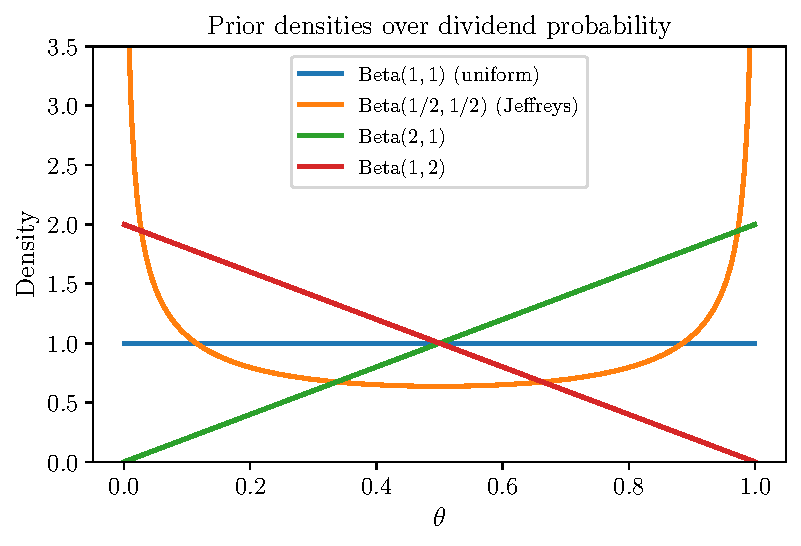
\includegraphics[width=0.55\textwidth]{morris_fig3_beta_priors.pdf}
\caption{Selected Beta densities over the dividend probability~$\theta$.}
\end{figure}

\end{frame}

% ──────────────────────────────────────────────────────────────────
\begin{frame}{Conjugate Updating}

After $t$ periods with $s$ dividend payments (successes):

\[
  \text{Prior: } \text{Beta}(a_i, b_i)
  \;\;\xrightarrow{\;s \text{ successes in } t \text{ trials}\;}
  \;\;\text{Posterior: } \text{Beta}(a_i + s,\; b_i + t - s).
\]

\medskip

\textbf{Posterior mean} (trader~$i$'s estimate of $\theta$):
\[
  \mu_i(s,t) \;=\; \E[\theta \mid s,t]
  \;=\; \frac{a_i + s}{a_i + b_i + t}.
\]

\medskip

Morris calls $\mu_i(s,t)$ trader~$i$'s \textbf{fundamental valuation}
after history $(s,t)$.

It is the probability trader~$i$ assigns to receiving a dividend next
period.

\end{frame}


% ══════════════════════════════════════════════════════════════════
\section{Market Prices with Learning}
% ══════════════════════════════════════════════════════════════════

\begin{frame}{Most Optimistic Valuation}

After history $(s,t)$, the \textbf{most optimistic fundamental
valuation} is:
\[
  \mu^*(s,t) \;=\; \max_{i \in \mathcal{I}}\; \mu_i(s,t).
\]

\medskip

The asset is held by the trader who assigns the \emph{highest}
value.

\medskip

An owner has the \textbf{option to sell} after receiving the
period's dividend---this option is priced into the equilibrium.

\end{frame}

% ──────────────────────────────────────────────────────────────────
\begin{frame}{Equilibrium Price}

The competitive equilibrium price (in current dollars) satisfies:
\[
  \tilde p(s,t,r) = \frac{1}{1+r}\Bigl[
    \mu^*(s,t)\bigl\{1 + \tilde p(s{+}1,t{+}1,r)\bigr\}
    + \bigl(1-\mu^*(s,t)\bigr)\,\tilde p(s,t{+}1,r)
  \Bigr].
\]

\medskip

\textbf{Normalized price:}
\[
  p(s,t,r) = r\,\tilde p(s,t,r).
\]

This is the price of the risky asset in terms of the riskless asset
(whose price is $1/r$).

\end{frame}

% ──────────────────────────────────────────────────────────────────
\begin{frame}{Normalized Price Recursion}

The normalized price satisfies:
\[
  p(s,t,r) \;=\; \frac{r}{1+r}\,\mu^*(s,t)
  + \frac{1}{1+r}\Bigl[
    \mu^*(s,t)\,p(s{+}1,t{+}1,r)
    + \bigl(1-\mu^*(s,t)\bigr)\,p(s,t{+}1,r)
  \Bigr].
\]

\medskip

Equivalently:
\[
  p(s,t,r) = \mu^*(s,t) + \frac{r}{1+r}\Bigl[
    \mu^*(s,t)\,p(s{+}1,t{+}1,r)
    + \bigl(1-\mu^*(s,t)\bigr)\,p(s,t{+}1,r) - \mu^*(s,t)
  \Bigr].
\]

\medskip

Computed via \textbf{value-function iteration}: set $p^0 \equiv 0$
and iterate
\[
  p^{n+1}(s,t,r) = \frac{r}{1+r}\,\mu^*(s,t)
  + \frac{1}{1+r}\Bigl[
    \mu^*(s,t)\,p^n(s{+}1,t{+}1,r)
    + \bigl(1-\mu^*(s,t)\bigr)\,p^n(s,t{+}1,r)
  \Bigr].
\]

\end{frame}

% ──────────────────────────────────────────────────────────────────
\begin{frame}{Speculative Premium}

When the identity of the most optimistic trader can \emph{switch}
with future dividend realizations:
\[
  p(s,t,r) > \mu_i(s,t) \quad \text{for \textbf{all} } i\in\mathcal{I}.
\]

\bigskip

The \textbf{speculative premium}:
\[
  p(s,t,r) - \mu^*(s,t) > 0.
\]

\bigskip

\begin{itemize}
\item The premium reflects the \textbf{option value} of reselling to
      whichever trader becomes temporarily more optimistic as
      dividends arrive.
\item It exists whenever there is \emph{no global optimist}.
\end{itemize}

\end{frame}


% ══════════════════════════════════════════════════════════════════
\section{Two-Trader Analysis}
% ══════════════════════════════════════════════════════════════════

\begin{frame}{Rate Dominance}

\begin{block}{Definition: Rate Dominance}
Trader~1 \textbf{rate-dominates} trader~2 if
\[
  a_1 \ge a_2 \quad\text{and}\quad b_1 \le b_2.
\]
\end{block}

\medskip

\begin{block}{Theorem: Global Optimist}
\begin{enumerate}
\item If trader~1 rate-dominates trader~2, then
      $\mu_1(s,t)\ge\mu_2(s,t)$ for all $(s,t)$.
      Trader~1 is a \textbf{global optimist}.
\item In this case $p(s,t,r) = \mu_1(s,t)$ and there is
      \textbf{no speculative premium}.
\end{enumerate}
\end{block}

\medskip

When \emph{neither} trader rate-dominates the other,
the identity of the most optimistic trader can switch
$\Rightarrow$ speculative premium.

\end{frame}

% ──────────────────────────────────────────────────────────────────
\begin{frame}{Posterior Means: Crossing vs.\ Non-Crossing}

\begin{figure}
\centering
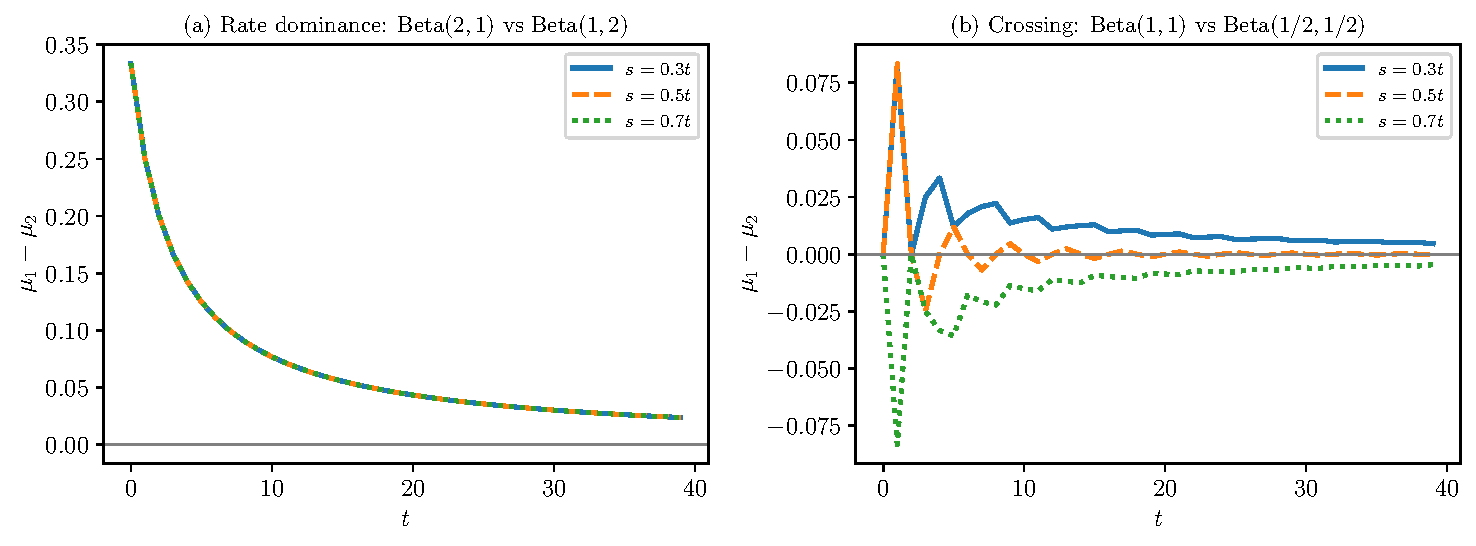
\includegraphics[width=0.82\textwidth]{morris_fig4_posterior_crossing.pdf}
\caption{(a)~Rate-dominant priors: $\mu_1 - \mu_2 > 0$ everywhere.
(b)~Non-dominant priors: posterior means cross, enabling
speculative premia.}
\end{figure}

\end{frame}


% ══════════════════════════════════════════════════════════════════
\section{Case A: Global Optimist}
% ══════════════════════════════════════════════════════════════════

\begin{frame}{Case A: Rate Dominance (No Premium)}

Priors: Trader~1 $\sim\text{Beta}(2,1)$, \;
Trader~2 $\sim\text{Beta}(1,2)$.

\medskip

Trader~1 rate-dominates ($a_1\ge a_2$, $b_1\le b_2$).

\medskip

\begin{center}
\renewcommand{\arraystretch}{1.3}
\begin{tabular}{ll}
\toprule
\textbf{Quantity} & \textbf{Value at $(s,t)=(0,0)$} \\
\midrule
$\tilde p(0,0)$ & $2.0$ \\
Fundamental value, trader~1 & $2.0$ \\
Fundamental value, trader~2 & $1.0$ \\
\bottomrule
\end{tabular}
\end{center}

\medskip

The price \textbf{exactly equals} trader~1's perpetuity value.

No speculative premium.

\end{frame}


% ══════════════════════════════════════════════════════════════════
\section{Case B: Perpetual Switching}
% ══════════════════════════════════════════════════════════════════

\begin{frame}{Case B: Perpetual Switching (Speculative Premium)}

Priors: Trader~1 $\sim\text{Beta}(1,1)$ (uniform), \;
Trader~2 $\sim\text{Beta}(1/2,1/2)$ (Jeffreys).

\medskip

Neither trader rate-dominates the other.

\medskip

\begin{center}
\renewcommand{\arraystretch}{1.3}
\begin{tabular}{ll}
\toprule
\textbf{Quantity} & \textbf{Value at $(s,t)=(0,0)$} \\
\midrule
$\tilde p(0,0)$ & $\approx 1.636$ \\
Fundamental value, trader~1 & $1.5$ \\
Fundamental value, trader~2 & $1.5$ \\
\bottomrule
\end{tabular}
\end{center}

\medskip

The price \textbf{exceeds both} traders' fundamental valuations.

The premium reflects the \textbf{option value} of reselling to
whichever trader becomes temporarily more optimistic.

\end{frame}


% ══════════════════════════════════════════════════════════════════
\section{Numerical Results}
% ══════════════════════════════════════════════════════════════════

\begin{frame}{Normalized Price vs.\ Interest Rate}

\begin{figure}
\centering
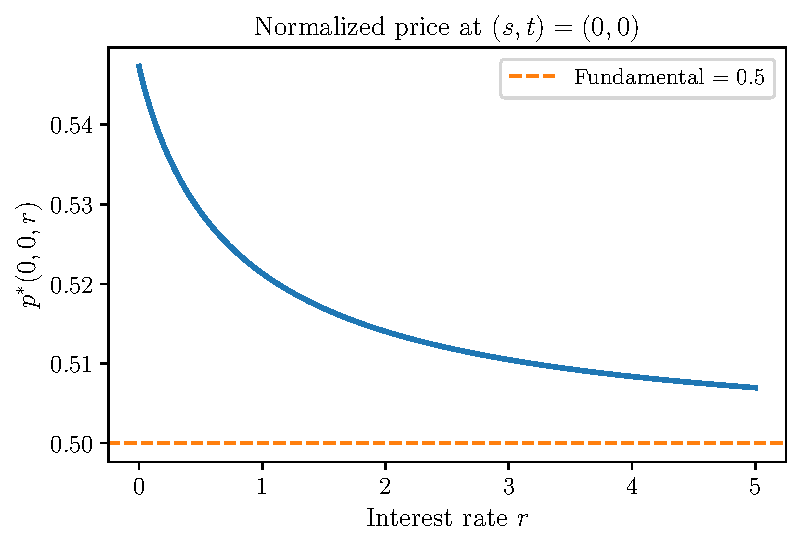
\includegraphics[width=0.65\textwidth]{morris_fig1_price_vs_r.pdf}
\caption{$p^*(0,0,r)$ as a function of $r$, for
$\text{Beta}(1,1)$ vs.\ $\text{Beta}(1/2,1/2)$.}
\end{figure}

\begin{itemize}
\item The resale option pushes $p^*(0,0,r)$ above the fundamental $0.5$
      for every finite~$r$.
\item As $r\to\infty$ ($\beta\to 0$), the option value fades  and
      $p^*\to 0.5$.
\item At $r=0.05$ the premium is about $8$--$9\%$.
\end{itemize}

\end{frame}

% ──────────────────────────────────────────────────────────────────
\begin{frame}{Normalized Price vs.\ Time}

\begin{figure}
\centering
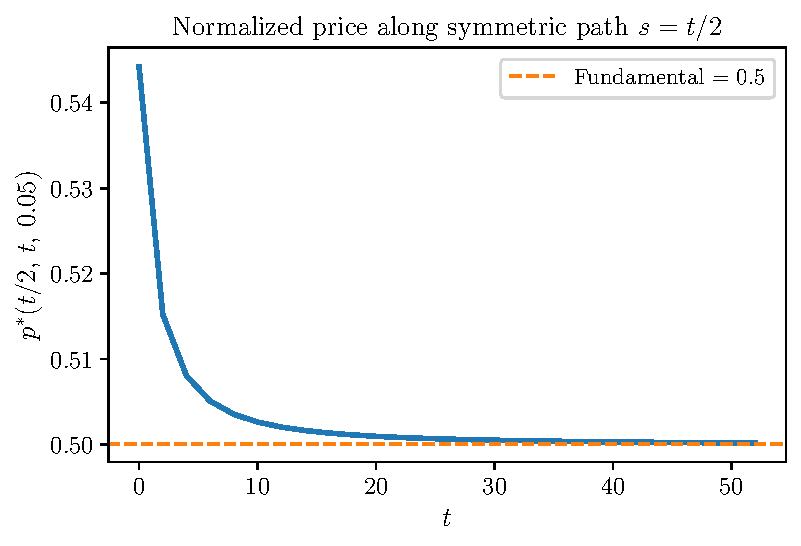
\includegraphics[width=0.65\textwidth]{morris_fig2_price_vs_t.pdf}
\caption{$p^*(t/2,\,t,\,0.05)$ along the symmetric path $s=t/2$.}
\end{figure}

\begin{itemize}
\item Along $s=t/2$, both traders' fundamentals equal $0.5$ at every~$t$.
\item Price starts above $0.5$ and declines toward $0.5$ as
      \textbf{learning reduces disagreement} and the resale option
      loses value.
\end{itemize}

\end{frame}

% ──────────────────────────────────────────────────────────────────
\begin{frame}{Speculative Premium Heat Map}

\begin{figure}
\centering
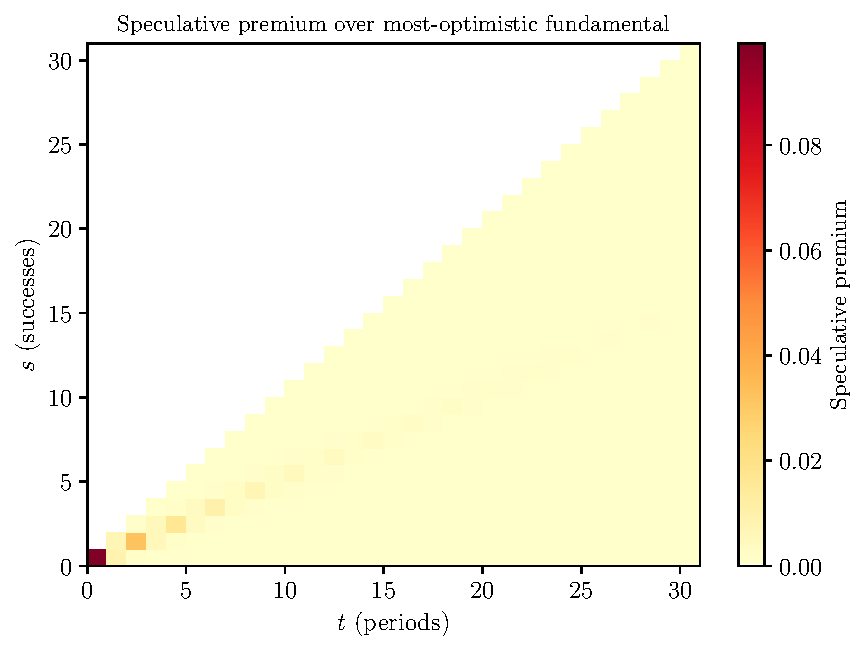
\includegraphics[width=0.55\textwidth]{morris_fig5_premium_heat.pdf}
\caption{Speculative premium over the most-optimistic fundamental
across histories $(s,t)$, $\beta=0.75$.}
\end{figure}

The premium is largest when $s\approx t/2$ (maximum  disagreement)
and shrinks as posteriors concentrate.

\end{frame}


% ══════════════════════════════════════════════════════════════════
\section{$N$--Trader Extension}
% ══════════════════════════════════════════════════════════════════

\begin{frame}{General $N$--Trader Case}

The recursion extends to any finite set of Beta priors
$\{(a_i,b_i)\}_{i=1}^N$ by taking a $\max$ over all $i$ at each
period:
\[
  \tilde p(s,t) = \beta \max_{i=1,\ldots,N}\Bigl[
    \mu_i(s,t)\bigl\{1+\tilde p(s{+}1,t{+}1)\bigr\}
    + \bigl(1-\mu_i(s,t)\bigr)\,\tilde p(s,t{+}1)
  \Bigr].
\]

\medskip

\textbf{Three-trader example} at $(s,t)=(0,0)$, $\beta=0.75$:

\begin{center}
\renewcommand{\arraystretch}{1.3}
\begin{tabular}{lcc}
\toprule
  & Prior & Fundamental value \\
\midrule
Trader 1 & $\text{Beta}(1,1)$ & $1.5$ \\
Trader 2 & $\text{Beta}(1/2,1/2)$ & $1.5$ \\
Trader 3 & $\text{Beta}(3,2)$ & $1.8$ \\
\midrule
\multicolumn{2}{l}{Asset price $\tilde p(0,0)$} & $\approx 1.96$ \\
\bottomrule
\end{tabular}
\end{center}

\medskip

No rate dominance $\Rightarrow$ price exceeds \emph{all} traders'
fundamental valuations $\Rightarrow$ speculative premium exists.

\end{frame}


% ══════════════════════════════════════════════════════════════════
\section{Rate Dominance \& Bubbles}
% ══════════════════════════════════════════════════════════════════

\begin{frame}{When Do Speculative Premia Arise?}

Morris (1996) provides a \textbf{sharp characterization}:

\bigskip

\begin{block}{Key Condition}
There is a \textbf{speculative premium} if and only if there is
\textbf{no global optimist}---i.e., no trader rate-dominates all others.
\end{block}

\bigskip

\textbf{Examples:}

\medskip
\begin{center}
\renewcommand{\arraystretch}{1.3}
\begin{tabular}{lcc}
\toprule
Priors & Rate dominance? & Premium? \\
\midrule
$\text{Beta}(2,1)$ vs.\ $\text{Beta}(1,2)$ & Yes (Trader 1) & No \\
$\text{Beta}(1,1)$ vs.\ $\text{Beta}(1/2,1/2)$ & No & Yes \\
$\text{Beta}(3,1),\;\text{Beta}(2,1),\;\text{Beta}(1,2)$ & Yes (Trader 1) & No \\
$\text{Beta}(1,1),\;\text{Beta}(1/2,1/2),\;\text{Beta}(3/2,3/2)$ & No & Yes \\
\bottomrule
\end{tabular}
\end{center}

\end{frame}

% ──────────────────────────────────────────────────────────────────
\begin{frame}{Checking Rate Dominance}

Trader~$i$ \textbf{rate-dominates} all others iff
\[
  a_i \ge a_j \quad\text{and}\quad b_i \le b_j
  \qquad\forall\; j \ne i.
\]

\medskip

\begin{itemize}
\item When this holds, $\mu_i(s,t)\ge\mu_j(s,t)$ for every
      history $(s,t)$.
\item Trader~$i$ is \emph{always} the most optimistic
      $\Rightarrow$ no switching $\Rightarrow$ no premium.
\item When it fails for every~$i$, switching occurs along some
      histories $\Rightarrow$ speculative bubble.
\end{itemize}

\end{frame}


% ══════════════════════════════════════════════════════════════════
\section{Concluding Remarks}
% ══════════════════════════════════════════════════════════════════

\begin{frame}{Concluding Remarks}

\begin{itemize}
\item Morris (1996) enriches   Harrison--Kreps (1978) by replacing
      dogmatic beliefs with \textbf{Bayesian learning}.

\item Speculative premia arise naturally when traders express
      ``maximal ignorance'' differently
      (e.g.\ uniform vs.\ Jeffreys prior).

\item The premium \textbf{declines over time} as posteriors
      merge---consistent with Miller's (1977) observation that IPO
      overpricing fades.

\item Key mechanism: the \textbf{option to resell} to a future
      optimist raises the price above \emph{every} trader's
      fundamental valuation.

\item The no-short-sales constraint is essential: if pessimists
      could short freely, the bubble would be arbitraged away.
\end{itemize}

\end{frame}

% ──────────────────────────────────────────────────────────────────
\begin{frame}{References}

\begin{thebibliography}{99}

\bibitem{HarrKreps1978}
Harrison, J.~M. and D.~M.~Kreps (1978).
\newblock Speculative investor behavior in a stock market with
heterogeneous expectations.
\newblock \emph{Quarterly Journal of Economics}, 92(2), 323--336.

\bibitem{Morris1996}
Morris, S. (1996).
\newblock Speculative investor behavior and learning.
\newblock \emph{Quarterly Journal of Economics}, 111(4), 1111--1133.

\bibitem{Miller1977}
Miller, E.~M. (1977).
\newblock Risk, uncertainty, and divergence of opinion.
\newblock \emph{Journal of Finance}, 32(4), 1151--1168.

\bibitem{Harsanyi1967}
Harsanyi, J.~C. (1967--68).
\newblock Games with incomplete information played by ``Bayesian''
players, Parts~I--III.
\newblock \emph{Management Science}, 14, 159--182, 320--334, 486--502.

\bibitem{Jeffreys1946}
Jeffreys, H. (1946).
\newblock An invariant form for the prior probability in estimation
problems.
\newblock \emph{Proceedings of the Royal Society~A}, 186, 453--461.

\end{thebibliography}

\end{frame}

\end{document}
